% \usepackage{amsmath}
% \usepackage{graphicx}
% \usepackage{tikz}


% ! /////////////////////////////
\documentclass[english, a4paper, 11pt]{article}

\usepackage{microtype}

\usepackage[T1]{fontenc}
\usepackage[utf8]{inputenc}

\usepackage{csquotes}
\usepackage{babel}

\usepackage{amsmath}
\usepackage{amsfonts}
\usepackage{amssymb}

\usepackage[bookmarks=true]{hyperref}
\hypersetup{
	pdftitle={Testosterone administration and },
	pdfauthor={Mohamad Rasoul Parsaeian},
	pdfkeywords={Social Hierarchy, single subject design},
	bookmarksnumbered,
	breaklinks=true,
	urlcolor=blue,
	citecolor=black,
	colorlinks=true,
	linkcolor=black,
}

\usepackage{lmodern}
\usepackage{amsmath}
\usepackage{amssymb}
\usepackage{textcomp}

\usepackage[style=ieee, citestyle=ieee]{biblatex}
\bibliography{references}

\usepackage[
	per-mode=symbol,
	%output-decimal-marker={,},
	separate-uncertainty=true,
]{siunitx}

\usepackage{booktabs}
\usepackage{caption}
\captionsetup[table]{skip=1ex}

\usepackage{tikz}
\usetikzlibrary{positioning}

\usepackage{graphicx}
\graphicspath{{figures/}}

\usepackage{pgfgantt}

\usepackage{cleveref}

\usepackage[
    % showframe,
	headheight=16mm,
    bottom=30mm,
]{geometry}

\usepackage{fancyhdr}
\fancypagestyle{unicamp}{
\renewcommand{\headrule}{}
\renewcommand{\footrule}{}
\fancyhead{}
\fancyfoot{}
\fancyhead[L]{\definecolor{unicampred}{RGB}{218,41,28}
\begin{tikzpicture}[x=0.08mm, y=0.08mm]
\fill (23.9531, 1.5) arc (3.58332:18.9167:24) -- (68.5957, 26.7897)arc (20.9142:16.5994:265.82) arc (128.381:171.373:10) -- cycle;
\fill (21.5557, 10.5523) arc (26.0833:41.4167:24) -- (55.0392, 52.9179)arc (32.5881:22.0609:144) -- cycle;
\fill (15.8767, 17.998) arc (48.5833:63.9167:24) -- (28.9371, 65.9407)arc (254.14:317.658:10) arc (56.8651:36.5278:55.38) -- cycle;
\fill (7.78063, 22.7038) arc (71.0833:86.4167:24) -- (1.5, 80.0404)arc (89.1258:74.8637:82.58) arc (170.647:236.876:10) -- cycle;
\fill (-1.5, 23.9531) arc (93.5833:108.917:24) -- (-28.6966, 73.1995)arc (115.826:92.2091:68.49) -- cycle;
\fill (-10.5523, 21.5557) arc (116.083:131.417:24) -- (-53.0458, 55.1671)arc (138.056:117.14:75.31) -- cycle;
\fill (-17.998, 15.8767) arc (138.583:153.917:24) -- (-67.7798, 29.6989)arc (162.818:139.707:66.11) -- cycle;
\fill (-22.7038, 7.78063) arc (161.083:176.417:24) -- (-67.7575, 1.5)arc (190.38:172.687:82.03) -- cycle;
\fill (-23.9531, -1.5) arc (183.583:198.917:24) -- (-56.342, -21.714)arc (214.771:200.588:92.45) -- cycle;
\fill (-21.5557, -10.5523) arc (206.083:221.417:24) -- (-38.6627, -36.5413)arc (237.639:225.296:92.84) -- cycle;
\fill (-15.8767, -17.998) arc (228.583:288.917:24) -- (13.0236, -35.3614)arc (118.011:187.497:10) arc (279.181:241.688:69.1) -- cycle;
\fill (10.5523, -21.5557) arc (296.083:311.417:24) -- (33.2593, -35.3806)arc (298.195:295.57:172.01) arc (31.6501:100.731:10) -- cycle;
\fill (17.998, -15.8767) arc (318.583:356.417:24) -- (71.3531, -1.5)arc (188.627:221.289:10) arc (312.84:298.995:193.11) -- cycle;
\fill[unicampred] (31.67, 75.56) circle (7);
\fill[unicampred] (81.24, 0) circle (7);
\fill[unicampred] (17.72, -44.19) circle (7);
\fill (-64, -80) -- (-64, -86.9041) .. controls (-63.9775, -89.3328) and (-63.9775, -89.3328) .. (-63.955, -89.8276) .. controls (-63.8426, -92.0315) and (-63.5952, -92.9535) .. (-62.8531, -93.7181) .. controls (-61.7286, -94.91) and (-59.9295, -95.2249) .. (-54.1949, -95.2249) .. controls (-50.7091, -95.2249) and (-49.2024, -95.1349) .. (-47.8531, -94.8651) .. controls (-46.1439, -94.5052) and (-44.997, -93.3133) .. (-44.7496, -91.6042) .. controls (-44.6147, -90.5472) and (-44.5922, -90.2999) .. (-44.5247, -86.9041) -- (-44.5247, -80) -- (-49.09, -80) -- (-49.09, -86.9041) .. controls (-49.09, -87.2189) and (-49.1124, -87.9385) .. (-49.1349, -88.4558) .. controls (-49.2024, -89.8726) and (-49.3148, -90.2774) .. (-49.6747, -90.6597) .. controls (-50.1694, -91.1994) and (-51.1139, -91.3343) .. (-54.2624, -91.3343) .. controls (-58.1529, -91.3343) and (-59.03, -91.087) .. (-59.2774, -89.8951) .. controls (-59.3898, -89.2879) and (-59.3898, -89.2654) .. (-59.4348, -86.9041) -- (-59.4348, -80) -- (-64, -80);
\fill (-41.2491, -80) -- (-41.2491, -95) -- (-36.5939, -95) -- (-36.7064, -83.8006) -- (-36.2116, -83.8006) -- (-28.3181, -95) -- (-20.3796, -95) -- (-20.3796, -80) -- (-25.0347, -80) -- (-24.9223, -91.1769) -- (-25.3945, -91.1769) -- (-33.2431, -80) -- (-41.2491, -80);
\fill (-17.0509, -80) -- (-17.0509, -95) -- (-12.2608, -95) -- (-12.2608, -80) -- (-17.0509, -80);
\fill (5.3068, -89.2204) .. controls (5.28431, -91.4468) and (5.21684, -91.4693) .. (0.201848, -91.4693) .. controls (-4.61075, -91.4693) and (-4.67821, -91.4243) .. (-4.67821, -87.5787) .. controls (-4.67821, -85.3073) and (-4.4983, -84.4303) .. (-3.95857, -83.9805) .. controls (-3.5088, -83.6207) and (-2.67671, -83.5307) .. (0.17936, -83.5307) .. controls (3.05792, -83.5307) and (4.38476, -83.6657) .. (4.72209, -83.958) .. controls (4.99195, -84.1829) and (5.03693, -84.3853) .. (5.08191, -85.3748) -- (9.64713, -85.3748) -- (9.64713, -84.6327) .. controls (9.64713, -82.2264) and (9.19735, -81.1244) .. (7.91549, -80.4723) .. controls (6.88101, -79.9325) and (5.48671, -79.7751) .. (1.48371, -79.7751) .. controls (-6.36487, -79.7751) and (-8.00655, -80.1574) .. (-8.81614, -82.1814) .. controls (-9.15348, -83.0135) and (-9.24343, -84.2504) .. (-9.24343, -87.6012) .. controls (-9.24343, -89.5127) and (-9.19845, -90.7496) .. (-9.13099, -91.4243) .. controls (-8.95108, -92.9535) and (-8.5013, -93.7856) .. (-7.51179, -94.3478) .. controls (-6.2974, -95.045) and (-4.40835, -95.2249) .. (1.46122, -95.2249) .. controls (4.78956, -95.2249) and (6.43124, -95.09) .. (7.64563, -94.7076) .. controls (9.30979, -94.1679) and (9.93948, -93.066) .. (9.93948, -90.6372) .. controls (9.93948, -90.4123) and (9.91699, -90.075) .. (9.8945, -89.2204) -- (5.3068, -89.2204);
\fill (29.0254, -95) -- (34.2203, -95) -- (26.3717, -80) -- (19.2653, -80) -- (11.3267, -95) -- (16.5441, -95) -- (17.826, -92.4588) -- (27.7435, -92.4588) -- (29.0254, -95) (26.1468, -89.1754) -- (19.4452, -89.1754) -- (22.3462, -83.4858) -- (23.2458, -83.4858) -- (26.1468, -89.1754);
\fill (36.1297, -80) -- (36.1297, -95) -- (40.6275, -95) -- (40.515, -83.7781) -- (41.3246, -83.7781) -- (46.9693, -95) -- (50.7699, -95) -- (56.4146, -83.7781) -- (57.1792, -83.7781) -- (57.0668, -95) -- (61.5645, -95) -- (61.5645, -80) -- (53.3336, -80) -- (48.8584, -89.7376) -- (44.4056, -80) -- (36.1297, -80);
\fill (64.896, -95) -- (69.4612, -95) -- (69.4612, -91.3343) -- (75.2183, -91.3343) .. controls (78.4567, -91.3343) and (79.4687, -91.2444) .. (80.4807, -90.907) .. controls (82.2798, -90.2549) and (82.887, -88.9505) .. (82.887, -85.6222) .. controls (82.887, -81.7766) and (82.0774, -80.5622) .. (79.2438, -80.1349) .. controls (78.4117, -80.0225) and (78.0069, -80) .. (75.1733, -80) -- (64.896, -80) -- (64.896, -95) (69.4612, -87.5787) -- (69.4612, -83.7556) -- (75.1733, -83.7556) .. controls (77.1748, -83.7781) and (77.2198, -83.7781) .. (77.5347, -83.8906) .. controls (78.1194, -84.093) and (78.3218, -84.5427) .. (78.3218, -85.6222) .. controls (78.3218, -86.6567) and (78.1868, -87.0615) .. (77.7596, -87.3313) .. controls (77.3772, -87.5562) and (77.2873, -87.5562) .. (75.1733, -87.5787) -- (69.4612, -87.5787);
\end{tikzpicture}
}
\fancyhead[C]{\sffamily%
{\bfseries\fontsize{15.5pt}{1em}\selectfont\uppercase{Universidade Estadual de Campinas}}\\
\fontsize{11.3pt}{1.2em}\selectfont\uppercase{Faculdade de Engenharia Elétrica e de Computação}\\
\uppercase{Departamento de Comunicações}}
\fancyfoot[C]{\sffamily\fontsize{9pt}{1em}\selectfont%
Av. Albert Einstein, 400; 13083-852 Campinas, SP, Brasil\\
Tel: +55 (19) 3521-3703; Fax: +55 (19) 3289-1395\\
\url{http://www.fee.unicamp.br}}
}

\pagestyle{plain}

\usepackage{setspace}

%\usepackage{parskip}

\usepackage{relsize}
\usepackage[nomain, acronym]{glossaries}
\setacronymstyle{long-sm-short}
\newcommand{\newacronymx}[8][]{%
	\newglossaryentry{#2}{
	type=\acronymtype,
	name={{\smaller #3}},
	sort={#3},
	first={#4 ({\smaller #3}, \emph{#5})},
	firstplural={#7 ({\smaller #6}, \emph{#8})},
	text={{\smaller #3}},
	plural={{\smaller #6}},
	description={#4 (\emph{#5})},#1}}

\newacronym{RTFM}{RTFM}{read the freaking manual}
\newacronymx{AOL}{AOL}{acronym in another language}{acrônimo em outra língua}{AOLs}{acronyms in another language}{acrônimos em outra língua}


% ! /////////////////////////////




\title{Behavioral and Physiological Consequences of Induced Changes in Social Hierarchies in Male Rats Using the Modified Food Competition Test and Cognitive Modeling via Dynamical Systems Theory: Interplay between Testosterone Administration and Food Access Alterations}
\author{Mohamad Rasoul Parsaeian}
\date{}

\begin{document}

\maketitle

\section*{Background}
Social hierarchies in rats can be influenced by various factors, including testosterone levels and access to food resources. Testosterone is known to increase aggression and dominance behaviors, while control over food resources can significantly affect social status.

\section*{Objectives}
\begin{enumerate}
    \item To investigate how the administration of testosterone and alterations in food access together affect the social hierarchy in triads of male rats.
    \item To assess the combined behavioral and physiological consequences of these interventions.
    \item To develop a dynamical systems model incorporating these factors to predict changes in social hierarchy.
\end{enumerate}

\section*{Hypotheses}
\begin{enumerate}
    \item Administration of testosterone will increase dominance behaviors and alter social hierarchies.
    \item Restricting food access for certain individuals will lead to increased competition and shifts in social status.
    \item The combination of testosterone administration and food access alteration will have a synergistic effect on social hierarchy dynamics.
\end{enumerate}

\section*{Methodology}
\subsection*{Participants}
40 adult male Sprague-Dawley rats, housed in groups of 3 (triads).

\subsection*{Interventions}
\begin{itemize}
    \item \textbf{Testosterone Administration}: Subordinate rats will receive testosterone injections (1 mg/kg body weight every 5 days).
    \item \textbf{Food Access Alteration}: Food access will be restricted for certain individuals within each triad to create competition.
\end{itemize}

\subsection*{Measurements}
\begin{itemize}
    \item \textbf{Social Hierarchy}: Determined using the modified Food Competition test.
    \item \textbf{Behavioral Analysis}: Observations of aggressive and submissive behaviors.
    \item \textbf{Physiological Metrics}: Corticosterone levels, body weight, immune function.
    \item \textbf{Cognitive Function}: Performance in maze tests and problem-solving tasks.
\end{itemize}

\subsection*{Procedure}
\begin{itemize}
    \item Establish baseline hierarchies using the modified Food Competition test.
    \item Apply testosterone administration and food access alterations.
    \item Monitor and record behavioral and physiological responses over 12 weeks.
\end{itemize}

\section*{Modified Food Competition Apparatus}

\begin{figure}[h]
    \centering
    \begin{tikzpicture}
        % Original image
        \node[inner sep=0pt] (image) at (0,0) {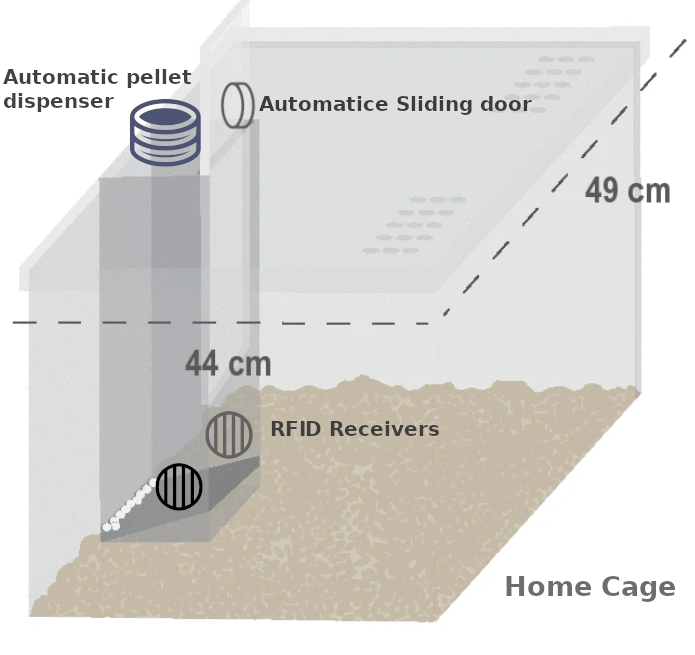
\includegraphics[width=0.8\textwidth]{figures/HomeCageModified.png}};

        % % Automatic Sliding Door
        % \draw[red, thick] (-3.5,-1) rectangle (-2,-2.5);
        % \node[red, below=of image, yshift=1.5cm, xshift=-2.5cm] {Automatic Sliding Door};

        % % RFID Receiver for Sliding Door
        % \draw[blue, thick] (-2,-1) circle (0.5);
        % \node[blue, below=of image, yshift=1.8cm, xshift=-1.8cm] {RFID Receiver};

        % % Automatic Pellet Release Mechanism
        % \draw[green, thick] (-6,-2) rectangle (-4.5,-3.5);
        % \node[green, below=of image, yshift=3.5cm, xshift=-5.5cm] {Automatic Pellet Release};

        % % RFID Receiver for Pellet Release
        % \draw[orange, thick] (-4.5,-2) circle (0.5);
        % \node[orange, below=of image, yshift=3.8cm, xshift=-4.3cm] {RFID Receiver};
    \end{tikzpicture}
    \caption{Schematic illustration of the home cage in the modified Food Competition apparatus.}
    \label{fig:modified_apparatus}
\end{figure}


\begin{figure}[h]
    \centering
    \begin{tikzpicture}
        % Original image
        \node[inner sep=0pt] (image) at (0,0) {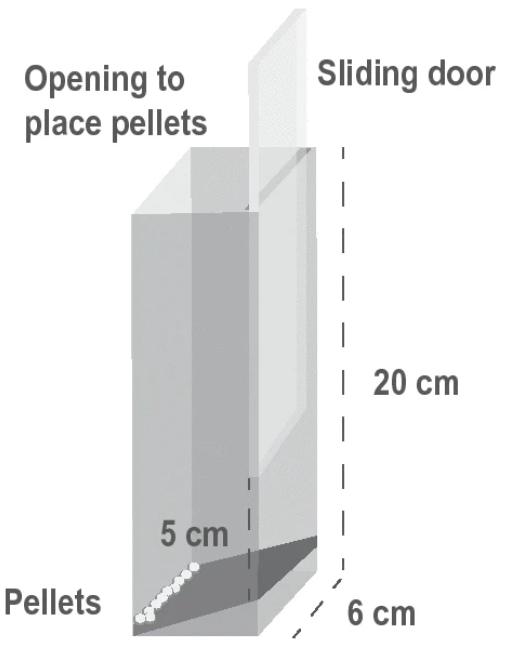
\includegraphics[width=0.8\textwidth]{figures/Feeder.png}};

        % % Automatic Sliding Door
        % \draw[red, thick] (-3.5,-1) rectangle (-2,-2.5);
        % \node[red, below=of image, yshift=1.5cm, xshift=-2.5cm] {Automatic Sliding Door};

        % % RFID Receiver for Sliding Door
        % \draw[blue, thick] (-2,-1) circle (0.5);
        % \node[blue, below=of image, yshift=1.8cm, xshift=-1.8cm] {RFID Receiver};

        % % Automatic Pellet Release Mechanism
        % \draw[green, thick] (-6,-2) rectangle (-4.5,-3.5);
        % \node[green, below=of image, yshift=3.5cm, xshift=-5.5cm] {Automatic Pellet Release};

        % % RFID Receiver for Pellet Release
        % \draw[orange, thick] (-4.5,-2) circle (0.5);
        % \node[orange, below=of image, yshift=3.8cm, xshift=-4.3cm] {RFID Receiver};
    \end{tikzpicture}
    \caption{Schematic illustration of the transparent lid and feeder in the modified Food Competition apparatus with modifications.}
    \label{fig:modified_apparatus_feeder}
\end{figure}
\begin{figure}[h]
    \centering
    \begin{tikzpicture}
        % Original image
        \node[inner sep=0pt] (image) at (0,0) {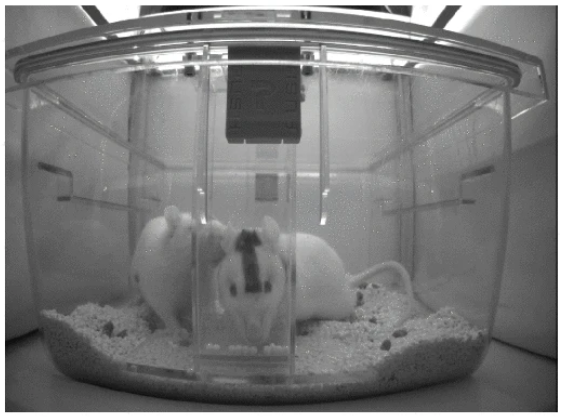
\includegraphics[width=0.8\textwidth]{figures/HomeCageInReality.png}};

        % % Automatic Sliding Door
        % \draw[red, thick] (-3.5,-1) rectangle (-2,-2.5);
        % \node[red, below=of image, yshift=1.5cm, xshift=-2.5cm] {Automatic Sliding Door};

        % % RFID Receiver for Sliding Door
        % \draw[blue, thick] (-2,-1) circle (0.5);
        % \node[blue, below=of image, yshift=1.8cm, xshift=-1.8cm] {RFID Receiver};

        % % Automatic Pellet Release Mechanism
        % \draw[green, thick] (-6,-2) rectangle (-4.5,-3.5);
        % \node[green, below=of image, yshift=3.5cm, xshift=-5.5cm] {Automatic Pellet Release};

        % % RFID Receiver for Pellet Release
        % \draw[orange, thick] (-4.5,-2) circle (0.5);
        % \node[orange, below=of image, yshift=3.8cm, xshift=-4.3cm] {RFID Receiver};
    \end{tikzpicture}
    \caption{Schematic illustration of the transparent lid and feeder in the modified Food Competition apparatus with modifications.}
    \label{fig:modified_apparatus_homecage_reality}
\end{figure}

\subsection*{Description of Modifications}

1. \textbf{Automatic Sliding Door}:
\begin{itemize}
    \item A motorized mechanism is installed to automate the sliding door.
    \item An RFID receiver is attached to recognize specific rats and control the door's opening.
\end{itemize}

2. \textbf{Automatic Pellet Release Mechanism}:
\begin{itemize}
    \item The pellet release mechanism is connected to a motorized system.
    \item An RFID receiver is integrated to control pellet release based on the rat's identification.
\end{itemize}

\subsection*{Automated Sliding Door and Pellet Dispenser System}

To study the behavioral and physiological consequences of induced changes in social hierarchies, we implemented an automated system to control access to food resources based on individual rat identification using RFID tags. This system consists of an automatic sliding door and a pellet dispenser, both responsive to RFID tags to ensure only specific rats can access the resources.

\subsubsection*{RFID Tagging}
\begin{itemize}
    \item Each rat is equipped with a unique RFID tag attached to its collar.
    \item The tags are pre-programmed to correspond to the identity of the subordinate or dominant status of each rat.
\end{itemize}

\subsubsection*{Automated Sliding Door}
\begin{itemize}
    \item The sliding door is equipped with a motorized mechanism controlled by a microcontroller.
    \item An RFID receiver is installed near the sliding door.
    \item When the RFID tag of a subordinate rat is detected by the receiver, the microcontroller activates the motor to open the door, allowing the rat to access the food area.
    \item If the RFID tag of a dominant rat is detected, the door remains closed.
\end{itemize}

\subsubsection*{Pellet Dispenser}
\begin{itemize}
    \item The pellet dispenser is similarly equipped with a motorized mechanism and an RFID receiver.
    \item Upon detecting the RFID tag of the subordinate rat, the dispenser releases a predetermined number of pellets.
    \item The dispenser remains inactive when the RFID tag of the dominant rat is detected, preventing access to additional food resources.
\end{itemize}

\subsubsection*{Experimental Procedure}
\begin{itemize}
    \item \textbf{Baseline Phase}: Initially, the social hierarchy within each triad of rats is determined using the modified Food Competition test.
    \item \textbf{Intervention Phase}: The automated system is activated, and the interactions between the rats are monitored. Subordinate rats are given exclusive access to additional food resources through the automated system.
    \item \textbf{Monitoring and Data Collection}: Behavioral observations are recorded, focusing on the frequency and duration of interactions with the sliding door and pellet dispenser. Physiological measures such as body weight and corticosterone levels are periodically assessed.
\end{itemize}

\subsubsection*{Data Analysis}
\begin{itemize}
    \item The data collected from the automated system is analyzed to determine changes in social hierarchy dynamics, food access patterns, and physiological responses.
    \item Statistical analyses are performed to compare the behavior and physiological measures between the subordinate and dominant rats.
\end{itemize}

By implementing this automated system, we ensure precise control over food resource allocation, allowing us to investigate the effects of altered food access on social hierarchy and related behavioral and physiological outcomes.

For more details, refer to the original research paper: \href{https://www.biorxiv.org/content/10.1101/2020.11.13.379719v1.full}{Behavioral and Physiological Consequences of Induced Changes in Social Hierarchies in Male Rats}.

\section*{Computational Cognitive Model}
\subsection*{State Variables}
\begin{itemize}
    \item \( S_i(t) \): Social status of rat \( i \) at time \( t \)
    \item \( A_i(t) \): Aggressiveness level of rat \( i \) at time \( t \)
    \item \( R_i(t) \): Resource access level of rat \( i \) at time \( t \)
    \item \( C_i(t) \): Corticosterone level of rat \( i \) at time \( t \)
    \item \( T_i(t) \): Testosterone level of rat \( i \) at time \( t \)
    \item \( F_i(t) \): Food access level of rat \( i \) at time \( t \)
\end{itemize}

\subsection*{Differential Equations}
\begin{align*}
    \frac{dS_i(t)}{dt} & = \beta A_i(t) + \xi E_i(t) - \eta D_i(t) - \epsilon (S_i(t) - \bar{S}(t)) + \phi T_i(t) + \lambda F_i(t)  \\
    \frac{dA_i(t)}{dt} & = \gamma C_i(t) + \phi T_i(t) - \epsilon (A_i(t) - \bar{A}(t)) + D \frac{\partial^2 A_i(t)}{\partial x^2}  \\
    \frac{dR_i(t)}{dt} & = \alpha S_i(t) - \epsilon (R_i(t) - \bar{R}(t)) + D \frac{\partial^2 R_i(t)}{\partial x^2}                \\
    \frac{dC_i(t)}{dt} & = \frac{1}{1 + \exp(-\theta (R_i(t) - S_i(t)))} - \delta C_i(t) + D \frac{\partial^2 C_i(t)}{\partial x^2} \\
    \frac{dT_i(t)}{dt} & = \text{Testosterone injection rate} - \delta T_i(t) + D \frac{\partial^2 T_i(t)}{\partial x^2}            \\
    \frac{dF_i(t)}{dt} & = \text{Rate of food access} - \delta F_i(t) + D \frac{\partial^2 F_i(t)}{\partial x^2}
\end{align*}

\section*{Expected Outcomes}
\begin{enumerate}
    \item Testosterone administration and food access alterations will lead to significant shifts in social hierarchy.
    \item Combined interventions will result in increased aggression, altered stress responses, and changes in cognitive performance.
    \item The dynamical systems model will accurately predict the effects of these interventions on social hierarchy dynamics.
\end{enumerate}

\section*{Significance}
This study will provide insights into the mechanisms through which hormonal and environmental factors influence social hierarchies and behavior. The findings will contribute to the understanding of social stress and hierarchy formation in animals, with potential implications for human social dynamics.

\end{document}
